\documentclass[tikz,border=2pt]{standalone}
\usepackage[T1]{fontenc}\usepackage[utf8]{inputenc}\usepackage{mathptmx}
\usepackage{pgfplots}\pgfplotsset{compat=1.18}
\pgfkeys{/pgf/number format/.cd,use comma,precision=2,fixed,fixed zerofill}
\definecolor{oscuro}{HTML}{4F7DB9}
\begin{document}
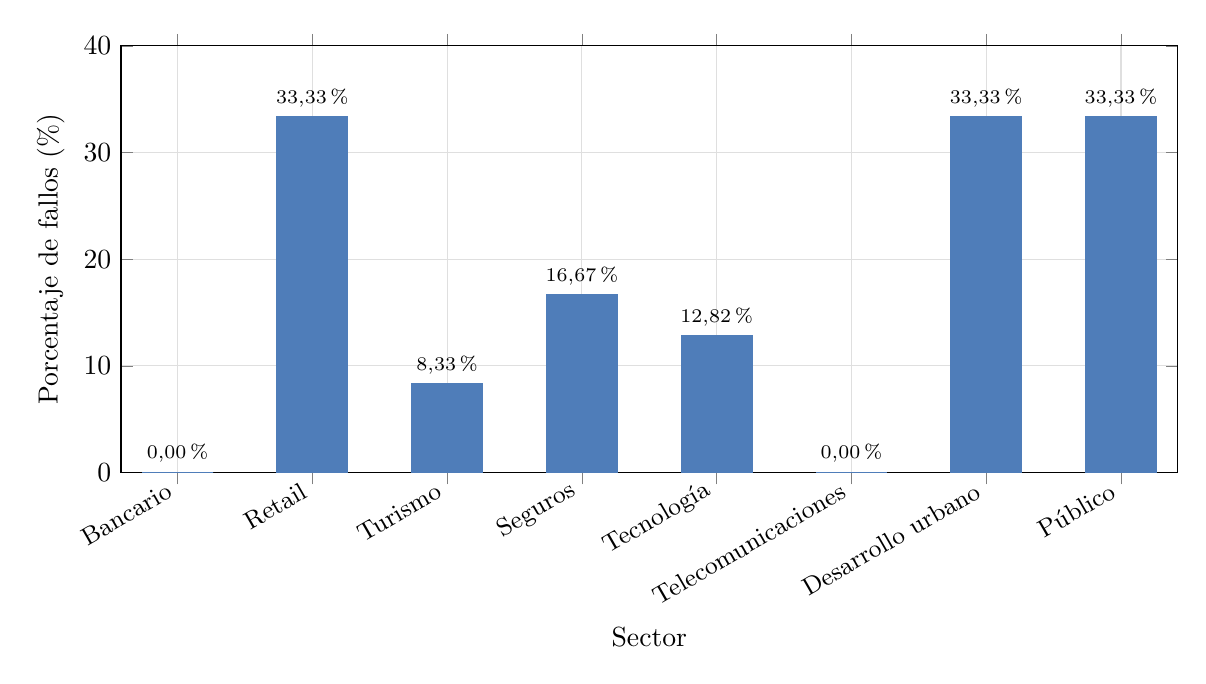
\begin{tikzpicture}
\begin{axis}[ybar, width=15cm, height=7cm, bar width=9mm, ymin=0, ymax=40,
  ylabel={Porcentaje de fallos (\%)}, xlabel={Sector}, symbolic x coords={Bancario,Retail,Turismo,Seguros,Tecnología,Telecomunicaciones,Desarrollo urbano,Público},
  xtick=data, enlarge x limits=0.06, ytick={0,10,20,30,40}, yticklabel={\pgfmathprintnumber[fixed,precision=0]{\tick}}, grid=major, grid style={gray!25},
  x tick label style={rotate=30, anchor=east, font=\small},
  nodes near coords={\pgfmathprintnumber[fixed,precision=2,fixed zerofill]{\pgfplotspointmeta}\,\%},
  every node near coord/.append style={font=\scriptsize}]
\addplot[fill=oscuro, draw=oscuro] coordinates {(Bancario,0.00) (Retail,33.33) (Turismo,8.33) (Seguros,16.67) (Tecnología,12.82) (Telecomunicaciones,0.00) (Desarrollo urbano,33.33) (Público,33.33)};
\end{axis}
\end{tikzpicture}
\end{document}
